\subsubsection{ Abstract Factory }

Il pattern \strong{ Abstract Factory } fornisce un'interfaccia per la creazione
di famiglie di oggetti correlati e dipendenti tra loro senza specificare le loro
classi concrete.

Il pattern può essere applicato quando

\begin{itemize}
  \item un sistema deve essere indipendente da come i suoi prodotti vengono
  creati, aggregati e rappresentati.
  \item un sistema deve interfacciarsi con molteplici famiglie di prodotti, dotate di
  interfaccia comune
  \item degli oggetti sono progettati per essere utilizzati insieme, e si vuole
  imporre tale vincolo
  \item si vuole esporre solo l'interfaccia di un gruppo di oggetti in una libreria di
  classi
\end{itemize}

\begin{figure}[h!]
  \centering
  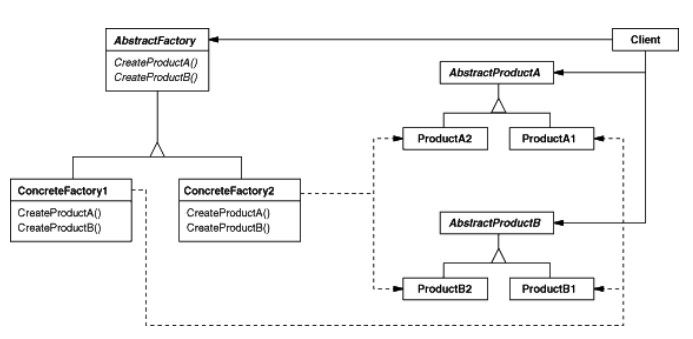
\includegraphics[scale=0.55]{imgs/abstract_factory.jpg}
  \caption{Diagramma delle classi del pattern Abstract Factory}
\end{figure}

Ogni famiglia di prodotti è creata da un'apposita ConcreteFactory, che il codice
client accede attraverso l'interfaccia di AbstractFactory. Solitamente, un solo
ConcreteFactory viene creato a run-time.

\paragraph{ Vantaggi }

\begin{enumerate}
  \item Classi concrete vengono isolate dal client
  \item È possibile cambiare la configurazione di prodotti semplicemente
    cambiando la ConcreteFactory che viene istanziata.
  \item Promuove consistenza tra i prodotti, imponendo che oggetti della stessa
    famiglia vengano usati insieme.
\end{enumerate}

\paragraph{ Svantaggi }

Tipicamente, l'interfaccia di AbstractFactory espone una serie di metodi
\emph{factory} che si occupano di costruire ogni oggetto della famiglia. Ogni
classe concreta specifica i suoi prodotti definendo l'implementazione di tali
metodi. Questa implementazione è semplice, ma ha lo svantaggio di richiedere un
una nuova ConcreteFactory e una completa ridefinizione dei metodi factory per
ogni famiglia di prodotti, anche se alcune famiglie differiscono tra loro solo
in alcuni dettagli.

Un altro svantaggio dell'Abstract Factory sta nella difficoltà di aggiungere
nuove classi di prodotti. L'interfaccia di AbstractFactory fissa l'insieme di
prodotti che possono essere creati, e aggiungerne di nuovi implica la modifica
della classe AbstractFactory e di tutte le ConcreteFactory che la ereditano.
